\preClass{Coordinate Systems}

\videoLink{Section 4.3}{https://www.youtube.com/playlist?list=PLYHZK3b8UFw2K5Q_epS1Wi1hezUGCYwtP}

\begin{enumerate}
\item  Find the exact values of the six trigonometric functions $\theta$ and $\alpha$.  Use the following triangle.


%\trigTriangle{$\theta$}{$\alpha$}{5}{}{2}

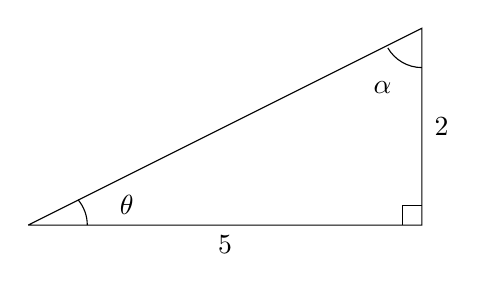
\begin{tikzpicture}[scale=2.5]
  \draw (0,0) -- (2,0) -- (2,1) -- (0,0);
  \draw (1.9,0) -- (1.9,0.1) -- (2,0.1);
  \draw (0.3,0) arc(0:40:0.2);
  \draw (0.5,0.1) node { $\theta$ };
  \draw (1.8,0.7) node { $\alpha$ };
  \draw (1,-0.1) node { 5 };
  \draw (1,0.6) node { ~ };
  \draw (2,0.8) arc(270:210:0.2);
  \draw (2.1,0.5) node { 2 };
\end{tikzpicture}


\begin{enumerate}
\begin{multicols}{2}
\item $\sin(\theta)=$\\[2.5em]
\item $\cos(\theta)=$\\[2.5em]
\item $\tan(\theta)=$\\[2.5em]
\item $\csc(\theta)=$\\[2.5em]
\item $\sec(\theta)=$\\[2.5em]
\item $\cot(\theta)=$\\[2.5em]

\columnbreak
\item $\sin(\alpha)=$\\[2.5em]
\item $\cos(\alpha)=$\\[2.5em]
\item $\tan(\alpha)=$\\[2.5em]
\item $\csc(\alpha)=$\\[2.5em]
\item $\sec(\alpha)=$\\[2.5em]
\item $\cot(\alpha)=$\\[2.5em]

\end{multicols}
\end{enumerate}

\clearpage

\item An observer at the top of a 462 ft mountain cliff measures the
  angle of depression from the top of the cliff to a point on the
  ground to be $5^\circ$.  What is the distance from the base (bottom)
  of the mountain to the point on the ground?  Round to the nearest
  foot. (Make a rough sketch of the situation clearly marking the
  relevant angles and distances before working out the problem.) If
  the angle of depression is a little bit bigger than $5^\circ$ will
  the distance increase or decrease? (Briefly justify your answer.)

  \vfill






\end{enumerate}



